\documentclass{article}
\usepackage[utf8]{inputenc}

\title{STL Notes}
\author{David Kooi}

\usepackage{float}
\usepackage{caption}
\usepackage{graphicx}
\usepackage{subfigure}
\usepackage{amssymb}
\usepackage{amsmath}
\usepackage{amsthm}
\usepackage{comment}
\usepackage{ragged2e}
\usepackage[margin=0.5in]{geometry}
\theoremstyle{definition}
\newtheorem{definition}{Definition}[section]

\begin{document}

\maketitle

\section{Autonomous Vehicles}
\subsection{Intersection Management}

\begin{figure}[H] 
\centering
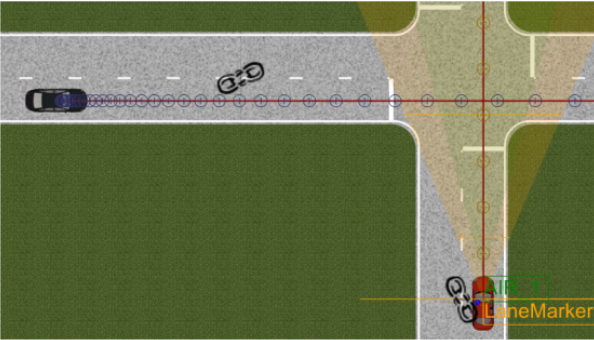
\includegraphics[width=2.5in]{Figures/raman_2015_intersection.png}
\caption{Intersection Scenario}
\label{fig:raman_intersection}
\end{figure}

In \cite{raman_reactive_2015} the ego-vehicle's behavior at an intersection is defined using STL. The system has a state: 
\begin{equation}
    \mathbf{x_t} = [x_{t}^{ego}\; y_{t}^{ego}\; x_{t}^{adv}\; y_{t}^{adv}\; v_{t}^{ego}\; v_{t}^{adv}\;]^T
\end{equation}

Figure \ref{fig:raman_intersection} shows the ego-vehicle in blue and the adversary-vehicle in red. The authors of \cite{raman_reactive_2015} use the following specification to describe the behavior: $\phi_s$: "When the ego-vehicle is within 2 meters of the adversary-vehicle the ego-vehicle will stop for two seconds."
\begin{equation}
    \phi_s = \square(|x_{t}^{ego} - x_{t}^{adv}| < 2) \implies \square_{[0,2]}(|v_{t}^{ego}|<0.1)
\end{equation}

\subsubsection{Alternate Formulation}
The above STL specification relies on the adversary-vehicle to stop at the intersection, but a car should always stop at an intersection. Inspired from \cite{chen_signal_nodate} the following specification describes: "When the ego-vehicle reaches an intersection it will stop for one second and only cross whens safe ($\phi_{cross}$) otherwise it will stay stopped. ($\phi_{stopped}\mathcal{U}_{[1,3]}\phi_{stopped}$)."

\begin{equation}
    \phi_{stopped} = (|v_{t}^{ego}|==0)
\end{equation}
\begin{equation}
    \phi_{cross} = \square_{[1,3]}(|y_{t}^{adv} - \mathbf{Y^{INT}}| > 0.1) \land (x_{t}^{ego} > 5)
\end{equation}

\begin{equation}
    \phi_{int} = \square(|x_{t}^{ego} -\mathbf{X^{INT}}|  < 0.1) \implies
    \square{[0.5,1]}(\phi_{stopped}) \land (\phi_{stopped}\mathcal{U}_{[1, 3]}\phi_{cross} \lor \phi_{stopped}\mathcal{U}_{[1,3]}\phi_{stopped})
\end{equation}

Where $\mathbf{X^{INT}} = -5$ and $\mathbf{Y^{INT}} = -5$
are the positional coordinates of the intersection.

\begin{figure}[H] 
\centering
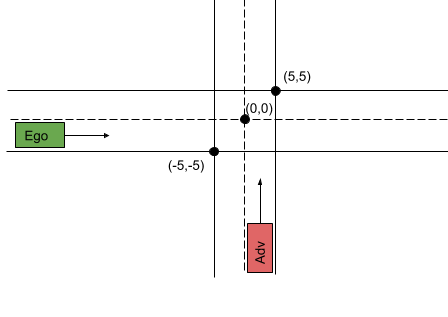
\includegraphics[width=2.5in]{Figures/intersection_stl.png}
\caption{Alternate Scenario}
\label{fig:alt_intersection}
\end{figure}


\section{STL for Hybrid Systems}

\subsection{Hybrid Time STL}
\subsubsection{Hybrid System Solutions}
Solutions to hybrid systems are defined on ordinary and discrete time:
\begin{enumerate}
    \item Ordinary Time: $t\in\mathbb{R}_{\geq0} :=  [0,\infty)$
    \item Discrete Time: $j\in\mathbb{N} := \{0,1,2,...\}$
\end{enumerate}
\begin{definition}[Hybrid Time Instance]
A \textit{hybrid time instance} is given by
\begin{center}
    $(t,j) \in \mathbb{R}_{\geq0} \times \mathbb{N}$
\end{center}
\end{definition}

\begin{definition}[Compact Hybrid Domain] A set $E \subset
    \mathbb{R}_{\geq0} \times \mathbb{N}$ is a  \textit{compact hybrid
    domain} if it can be written as
\begin{equation}
    \label{eq:compact_htd}
    E = \bigcup\limits_{j=0}^{J-1} ([t_j,t_{j+1}] \times \{j\}
\end{equation}
for a finite sequence of times $0 = t_0 \leq t_1 \leq t_2 \leq ... \leq t_J$.
\end{definition}

\begin{definition}[Hybrid Domain]
A set $E \subset \mathbb{R}_{\geq0} \times \mathbb{N}$ is a \textit{hybrid  domain} if for each $(T,J)\in\;E$
\begin{center}
    $E \cap ([0,T] \times \{0,1,...,J\}$
\end{center} 
is a compact hybrid time domain.
\end{definition}

\begin{definition}[Compact Hybrid Shift] Given a compact hybrid domain $E$
    and $(t^*,j^*)$, the forward {compact hybrid shift} of $E$ by $(t^*,j^*)$ is
\begin{equation}
    (t^*,j^*) + E = \bigcup\limits_{j=0}^{J-1} ([t_j + t^*,t_{j+1}+t^*] \times \{j+j^*\}\quad\\
\end{equation}
and the backward hybrid shift of $E$ by $(t^*,j^*)$ is
\begin{equation}
    E - (t^*,j^*) = \bigcup\limits_{j=0}^{J-1} ([t_j - t^*,t_{j+1}-t^*] \times \{j-j^*\}\\
\end{equation}
for a finite sequence of times $0 = t_0 \leq t_1 \leq t_2 \leq ... \leq t_J$
and E satisfying (\ref{eq:compact_htd}).
\end{definition}

\begin{definition}[Compact hybrid Interval] A \textit{compact hybrid
    interval} is defined by two hybrid time instances $(t^*_A,j^*_A)$ and
    $(t^*_B,j^*_B)$, where $t^*_A + j^*_A \leq t^*_B + j^*_B$, and an hybrid domain $E$, over the range $[t^*_A,
    t^*_B]\times\{j^*_A,..., j^*_B\}$, by

\begin{gather}
    \mathcal{I} := (t^*_A,j^*_A) + E = \bigcup\limits_{j=0}^{J-1} ([t_j + t^*_A,t_{j+1} + t^*_A] \times \{j + j^*_A\}
\end{gather}

Where $J = j^*_B - j^*_A$ and $t_0 = 0 \leq t_1 \leq t_2 \leq ... \leq t_J = t^*_B - t^*_A$
\end{definition}

\begin{definition}[Open Hybrid Interval]
An open hybrid interval is defined by two hybrid time instances,
$(t^*_A,j^*_A)$ and $(t^*_B,j^*_B)$, on hybrid domain $E$, over the
range $[t^*_A, t^*_B]\times\{j^*_A,..., j^*_B\}$, by the following cases:

\begin{enumerate}
    \item Left open interval
    \begin{gather}
        \mathcal{I} := (t^*_A, t_1] \times \{j^*_A\} \cup
        \bigcup\limits_{j=1}^{J-1} ([t_j+t^*_A,t_{j+1}+t^*_A] \times \{j+j^*_A\} 
    \end{gather}
    Where $J = j^*_B - j^*_A$ and $t_0 = 0 \leq t_1 \leq t_2 \leq ... \leq t_J = t^*_B - t^*_A$

    \item Right open interval
    \begin{equation}
        \mathcal{I} :=  \bigcup\limits_{j=0}^{J-2} ([t_j+t^*_A,t_{j+1}+t^*_A] \times \{j+j^*_A\} 
                         \cup [t_{J-1}, t^*_B) \times \{j^*_B\}
    \end{equation}
    Where $J = j^*_B - j^*_A$ and $t_0 = 0 \leq t_1 \leq t_2 \leq ... \leq t_J = t^*_B - t^*_A$
\end{enumerate}

\end{definition}


\clearpage
\begin{flushleft}
\textbf{Remark:}
Authors of \cite{hutchison_robust_2010} denote a ordinary time interval $\mathcal{I}$, relative to ordinary time $t$ as: 
\end{flushleft}

\begin{center}
$t + \mathcal{I} := \{t+t': t' \in \mathcal{I}\}$ 
\end{center}
The same notation can be used denoting a hybrid temporal interval, $\mathcal{I}$ relative to hybrid time instance $(t,j)$:
\begin{center}
    $(t,j) + I := \{(t+t',j+j'): (t',j') \in I\}$
\end{center}


\clearpage
\subsection{Continuous Time STL}
A STL formula $\phi$ is defined recursively as:
\begin{equation}
    \psi ::= p^\mu\;|\;\lnot \psi\;|\;\psi_1 \land \psi_2\;|\;\lozenge_{\mathcal{I}} \psi\;|\;\psi_1 U_{\mathcal{I}} \psi_2
\end{equation}


Where $\psi_1$, $\psi_2$ are STL formula and $\mathcal{I}$ is an ordinary time interval of form $\mathcal{I} = (t_a,t_b),(t_a,t_b],[t_a,t_b),$ or $[t_a,t_b]$ with $t_a < t_b$ and $\mathcal{I} \subset \mathbb{R}_{\geq 0}$.

\begin{center}
    Inductive STL Definition
\end{center}
\begin{alignat*}{3}
            &\phi \models \psi &&\Leftrightarrow (\phi, t) \models p \\
            &(\phi, t) \models p^\mu \quad &&\Leftrightarrow \mu(\phi(t))
> 0\\
            &(\phi, t) \models \square_{[a,b]} \psi &&\Leftrightarrow
\forall t' \in [t + a, t + b]\;s.t\;(\phi, t') \models \psi
\end{alignat*}



\begin{comment}
\begin{definition}[Compact Hybrid Interval]
A \textit{compact hybrid interval} $\mathcal{I}$ is defined by two hybrid time instances $(t^*_1, j^*_1)$ and $(t^*_2, j^*_2)$ on a compact hybrid time domain $E$.
\begin{equation}
    \mathcal{I} := E - (t^*_1,j^*_1) \cap [0, T^*] \times \{0,1,...,J^*\}
\end{equation}
Where $t^*_1 \leq t^*_2$, $j^*_1 \leq j^*_2$, $T^* = t^*_2 - t^*_1$ and $J^* = j^*_2 - j^*_1$
\end{definition}
\end{comment}

\begin{comment}
\begin{flushleft}
\textbf{Example}
Let $E = [0, 10] \times {0}$ be a compact hybrid time domain. Let the upper and lower limits of interval $\mathcal{I}$ be $(2,0)$ and $(5,0)$. Then, 

    \begin{align*}
        \mathcal{I} &= E - (2,0) \cap [0, 3] \times {0}\\
                    &= [-2,8] \cap [0,3]\\
                    &= [0,3]
    \end{align*}
\end{flushleft}
\end{comment}


\clearpage


\subsubsection{Possible Notion of Hybrid STL}
\begin{center}
    Recursive STL Definition
\end{center}
\begin{equation}
    \psi ::= p^\mu\;|\;\lnot \psi\;|\;\psi_1 \land \psi_2\;|\;\lozenge_{I} \psi\;|\;\psi_1 U_{I} \psi_2
\end{equation}
Where $\psi_1$, $\psi_2$ are STL formula and $I$ is a hybrid time interval.

\begin{center}
    Inductive STL Definition
\end{center}
\begin{alignat*}{3}
            &\phi \models \psi &&\Leftrightarrow (\phi, (t,j)) \models p \\
            &(\phi, (t,j) \models p^\mu \quad &&\Leftrightarrow \mu(\phi(t))
> 0\\
            &((\phi,(t,j)) \models \square_{I} \psi &&\Leftrightarrow \forall (t',j') \in (t,j)+I\;s.t.\;(\phi, (t',j')) \models \psi
\end{alignat*}


\begin{comment}
\begin{equation}
            ((\phi,(t,j)) \models \square_{I} \psi \Leftrightarrow \forall (t+t',j+j') \in I' ,(t+t',j+j') \in dom\phi\;s.t\;(\phi, (t+t',j+j')) \models \psi\;,\; I' = [t + t_a, t + t_b] \times [j + j_a, j + j_b]
\end{equation}
\end{comment}





\subsubsection{Previous Notions of Hybrid STL}
From Atreya - Modeling Hybrid Systems using Signal Temporal Logic
\begin{center}
    Inductive STL Definition
\end{center}

\begin{equation}
            ((\phi,(t,j)) \models \square_{(t,j)} \psi \Leftrightarrow \forall (t',j') \in dom\;\phi, t'+j' > t + j\;s.t\;(\phi, (t',j')) \models \psi
\end{equation}




\clearpage
\appendix
\subsection{Lane Changing}
The authors of \cite{chen_signal_nodate} use STL and Hamilton Jacobi reachability to combine temporal specification with quantification of a reachable set: STL temporal specifications are related to reachability operators.

\subsubsection{Example}
\begin{figure}[H] 
\centering
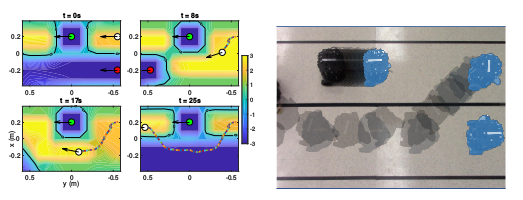
\includegraphics[width=4.5in]{Figures/chen_lanechange.png}
\caption{Lane Change Scenario}
\label{fig:chen_lane_change}
\end{figure}
In Figure \ref{fig:chen_lane_change} white represents the autonomous car, green a slow car, and red an adjacent car. The white car's lane change specification is given as: "Within 25 seconds, satisfy general safety $\phi$ until you can pass. Otherwise stay within the lane. Also ensure you are always within 5 seconds from re-entering the lane.($\psi^{lane}$.)"

\begin{equation}
    \phi = \phi^{off-road} \land \phi^{on-road} \land \phi^{avoid} 
\end{equation}

\begin{equation}
    \square_{[0,25]}\lozenge_{[0,5]}\psi^{lane} \land (\phi\mathcal{U}_{[0,25]}\psi^{pass} \lor \phi\mathcal{U}_{[0,25]}\psi^{stay})
\end{equation}


\subsection{Solutions for Discrete Systems}
Consider a discrete system of the form:
\begin{equation}
    x^{+} \in G(x,\gamma)
\end{equation}
Let $x \in \mathbb{R}^n$ be states of the discrete system.\\
Let $\gamma \in \mathbb{R}^m$ be input to the discrete system. \\
Discrete time is denoted: $k \in \mathbb{N}$\\
Then, given an initial state, $x_0$ and an input $k \mapsto \gamma(k)$, a state trajectory(solution)
can be constructed. The domain of $\gamma$ is given: $dom\;\gamma = \{0,1,2,...,K\}\cap \mathbb{N}$ where $K \in \mathbb{N} \cup \{\infty\}$. Solutions are defined as: $k \mapsto \phi(k)$ such that the following are satisfied:
\begin{enumerate}
    \item $\phi(0) = x_0$
    \item $dom\;\phi = dom\;\gamma$ if $K=\infty$
    \item $dom\;\phi \setminus \{max\; dom\;\phi\} = dom\;\gamma$ if $K$ is finite
    \item $\forall k \in dom\;\gamma$: $\phi(k+1) = G(\phi(k),\gamma(k))$
\end{enumerate}
\subsubsection{Discrete Time STL}
\begin{equation}
    \psi ::= p^\mu\;|\;\lnot \psi\;|\;\psi_1 \land \psi_2\;|\;\lozenge_{I} \psi\;|\;\psi_1 U_{I} \psi_2
\end{equation}
Where $\phi_1$, $\phi_2$ are STL formula and $I$ is an interval on $dom\;\phi$.

\begin{center}
    Inductive STL Definition
\end{center}
\begin{alignat*}{3}
            &\sigma \models \psi &&\Leftrightarrow (\sigma, k) \models p \\
            &(\sigma, k) \models p^\mu \quad &&\Leftrightarrow \mu(x_k, \gamma_k) > 0\\
            &(\sigma, k) \models \square_{[n,m]} \psi &&\Leftrightarrow \forall k' \in [k' + n, k' + m]\;s.t\;(\sigma, k') \models \psi
\end{alignat*}




\bibliographystyle{IEEEtran}
\bibliography{ref}

\end{document}
